\documentclass{article}
\usepackage{tikz, comment}
\usepackage{pifont}
\usepackage{fontspec, pgfplots}
\usetikzlibrary{arrows, decorations.markings, decorations.pathreplacing}
\begin{comment}
:Title: Not defined yet
:Tags: moment;focus of a parabola;directrix of a parabola;parabola;apothem
:Prob: 0.6278;0.6215;0.6121;0.6017;0.5934
:Author: Prof.Hu Ji-shan, HKUST
:Slug: No name yet

Description Here.........
\end{comment}
\begin{document}\centering 

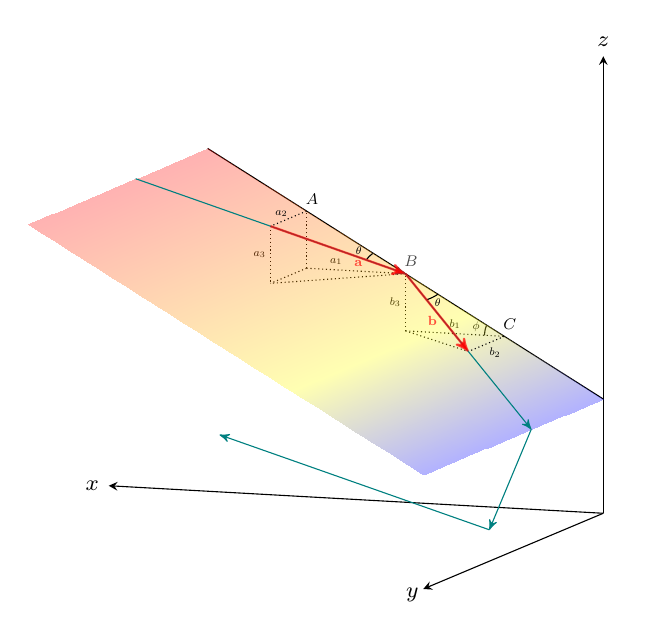
\begin{tikzpicture}[font=\footnotesize]
\pgfplotsset{compat=1.8}
\begin{axis}
[axis lines = center, view={200}{10}, ticks=none, no marks, scale=1.25,
axis background, xlabel = {$x$}, ylabel ={$y$}, zlabel ={$z$}, domain =-2:2, y domain =-2:2,
xmin =0,
xmax =5,
ymin =0,
ymax =5,
zmin =0, 
zmax =4,
samples =10, samples y =40, z buffer = auto, 
every axis x label/.style={
    at={(ticklabel* cs:1)},
    anchor= east, yshift =0
},
every axis y label/.style={
    at={(ticklabel* cs:1)},
    anchor= south, xshift = -4, yshift = -8
},
every axis z label/.style={
    at={(ticklabel* cs:1)},
    anchor= south
}]

\addplot3[black] coordinates {(0,0,1) (4,0,3)}; %z=1+0.5x, y=0

\addplot3[densely dotted] coordinates {(3,0,2.5) (3,0,2)} ;
\addplot3[densely dotted] coordinates {(3,1,2) (3,0,2)} ;
\addplot3[densely dotted] coordinates {(3,1,2) (3,1,2.5)} 
node[black, left, midway, pos=0.5, xshift=0, yshift=0, scale=0.5]{$a_3$}; 

\addplot3[densely dotted] coordinates {(3,1,2) (2,0,2)} ; 
\addplot3[densely dotted] coordinates {(2,0,2) (3,0,2)} 
node[black, above, midway, pos=0.3, xshift=0, yshift=0, scale=0.5]{$a_1$}; 
 
\addplot3[densely dotted] coordinates {(1,0,1.5) (2,0,1.5)}
node[black, above, midway, pos=0.5, xshift=0, yshift=0, scale=0.5]{$b_1$};

\addplot3[densely dotted] coordinates {(2,0,2) (2,0,1.5)}
node[black, left, midway, pos=0.5, xshift=0, yshift=0, scale=0.5]{$b_3$}; 

\addplot3[densely dotted] coordinates {(1,1,1.5) (2,0,1.5)}; 

\addplot3 [data cs=cart, black, samples=40, domain=0:25, y domain = 0:0] ({1+0.2*cos(x)},{0},{1.5+0.2*sin(x)})node[black, left, xshift=0, yshift=3, scale=0.5]{$\phi$};

\addplot3[surf, opacity=0.3, shader=interp, samples=40, domain=0:4, y domain = 0:5, z buffer=sort] ({x},{y},{1+0.5*x});%the plane

\addplot3[densely dotted] coordinates {(3,1,2.5) (3,0,2.5) }
node[black, above, midway, pos=0.7, xshift=0, yshift=0, scale=0.5]{$a_2$}
node[black, above, midway, pos=0, xshift=2, yshift=0, scale=0.7]{$A$};
 
\addplot3[densely dotted] coordinates {(1,1,1.5) (1,0,1.5)}
node[black, right, midway, pos=0.7, xshift=2, yshift=-2, scale=0.5]{$b_2$}
node[black, above, midway, pos=0, xshift=2, yshift=0, scale=0.7]{$C$};  

\addplot3 [data cs=cart, black, samples=40, domain=25:40, y domain = 0:0] ({2+0.5*cos(x)*cos(30)},{0},{2+0.5*sin(x)*sin(30)})node[black, left, xshift=0, yshift=3.3, scale=0.5]{$\theta$};

\addplot3 [data cs=cart, black, samples=40, domain=220:240, y domain = 0:0] ({2+0.5*cos(x)*cos(30)},{0},{2+0.5*sin(x)*sin(30)})node[black, right, xshift=-3, yshift=-3, scale=0.5]{$\theta$};

\addplot3[teal, <-, >=stealth'] coordinates {(4,2,3) (2,0,2) }; %z=1+0.5x, y=0

\addplot3[teal, ->, >=stealth'] coordinates {(0,2,1) (2,0,2)}; %(0,2,1)=(2,0,2) + (1)[(2,0,2) - (4,-2,3)]

\addplot3[teal, <-, >=stealth'] coordinates {(0,2,1) ({-2*(-1/3)}, {2+2*(-1/3)}, {1+3*(-1/3)})  }; %(-2s,2+2s,1+3s)=(0,2,1) + (s)[(0,2,1)-(2,0,-2)]

\addplot3[teal, ->, >=stealth'] coordinates {({-2*(-1/3)+2*(1)}, {2+2*(-1/3)+2*(1)}, {1+3*(-1/3)+1*(1)}) ({-2*(-1/3)}, {2+2*(-1/3)}, {1+3*(-1/3)}) }; %()=({-2*(-1/3)}, {2+2*(-1/3)}, {1+3*(-1/3)}) + (s)[(0,2,1)-(2,0,-2)]

\addplot3[red, thick, opacity=0.7, <-, >=stealth'] coordinates {(3,1,2.5) (2,0,2) }
node[below, midway, pos=0.35, xshift=0, yshift=1, scale=0.6]{${\bf a}$}
node[black, above, midway, pos=0, xshift=2, yshift=0, scale=0.7]{$B$}; 

\addplot3[red, thick, opacity=0.7, ->, >=stealth'] coordinates {(1,1,1.5) (2,0,2) }
node[left, midway, pos=0.6, xshift=0, yshift=0, scale=0.6]{${\bf b}$}; 

\end{axis}

\end{tikzpicture}
\end{document}